\documentclass[14pt,aspectratio=169]{beamer}

\usepackage{pgfpages}
\usepackage{fancyvrb}

\usepackage{tikz}
\usepackage{pgfplots}

\usepackage{minted}
\usemintedstyle{tango}

\usepackage{graphicx}

\usetheme{auriga}
\usecolortheme{auriga}

\setbeamercolor{background canvas}{bg=lightgray}

% define some colors for a consistent theme across slides

\definecolor{red}{RGB}{181, 23, 0}
\definecolor{blue}{RGB}{0, 118, 186}
\definecolor{gray}{RGB}{146, 146, 146}

\title{Web Development: \\ Effective Web Page Layout}

\author{{\bf Gregory M. Kapfhammer}}

\institute[shortinst]{{\bf Department of Computer Science, Allegheny College}}

\begin{document}

{
  \setbeamercolor{page number in head/foot}{fg=background canvas.bg}
  \begin{frame}
    \titlepage
  \end{frame}
}

% Slide
%
\begin{frame}{Technical Question}
  %
  \hspace*{.25in}
  %
  \vspace*{.2in}
  %
  \begin{minipage}{4.5in}
    %
    \begin{center}
      %
      {\large How can I leverage my understanding of the fundamentals of
      JavaScript to add interactivity to a web page with functions, arrays, and
      objects?}
      %
    \end{center}
    %
  \end{minipage}
  %
  \vspace{2ex}
  %
  \begin{center}
    %
    \small Let's learn how to combine HTML, CSS, and JavaScript to create
    interactive web pages! Since this material assumes a knowledge of web pages,
    please review all previous content about mobile-ready web development! \\
    %
  \end{center}
  %
\end{frame}

% Slide
%
\begin{frame}{The Normal Flow of Web Page Layout}
  %
  \begin{itemize}
    %
    \item How does the web browser normally layout the block-level and inline
      elements from left to right and top to bottom?
      %
      \vspace*{-.15in}
      %
    \item The fundamental components of a web page:
      %
      \begin{itemize}
        %
        \item {\bf Block-level elements}: content contained on their own line
          %
        \item {\bf Inline elements}: content displayed within an existing line
          %
          \begin{itemize}
            %
            \item {\bf Replaced}: content defined by an external resource
              %
            \item {\bf Non-replaced}: content defined by an in-document
              resources
              %
          \end{itemize}
          %
      \end{itemize}
      %
      \vspace*{-.2in}
      %
    \item How can you tell if a component is block-level or not?
      %
      \vspace*{-.2in}
      %
    \item How can you tell if a component is inline or not?
      %
      \vspace*{-.2in}
      %
    \item When is an element replaced versus non-replaced?
      %
  \end{itemize}
  %
\end{frame}

% Slide
%
\begin{frame}[fragile]
  \frametitle{Identifying Block-Level and Inline Content}
  \normalsize
  \begin{minipage}{6in}
    \vspace*{.1in}
    \begin{minted}[mathescape, numbersep=5pt, fontsize=\large]{html}
<h3>Photograph Reviews</h3>
<blockquote>
  <p><b>By Ricardo on
     <time>February 8, 2018</time></b>
  </p>
  <p>That is a great photograph!</p>
  <p>I would describe this as
     <i class="em em---1"></i></p>
</blockquote>
    \end{minted}
  \end{minipage}
%
\end{frame}

% Slide
%
\begin{frame}{Responsive Web Debugging with Firefox}
  %
  \begin{figure}
    \centering
    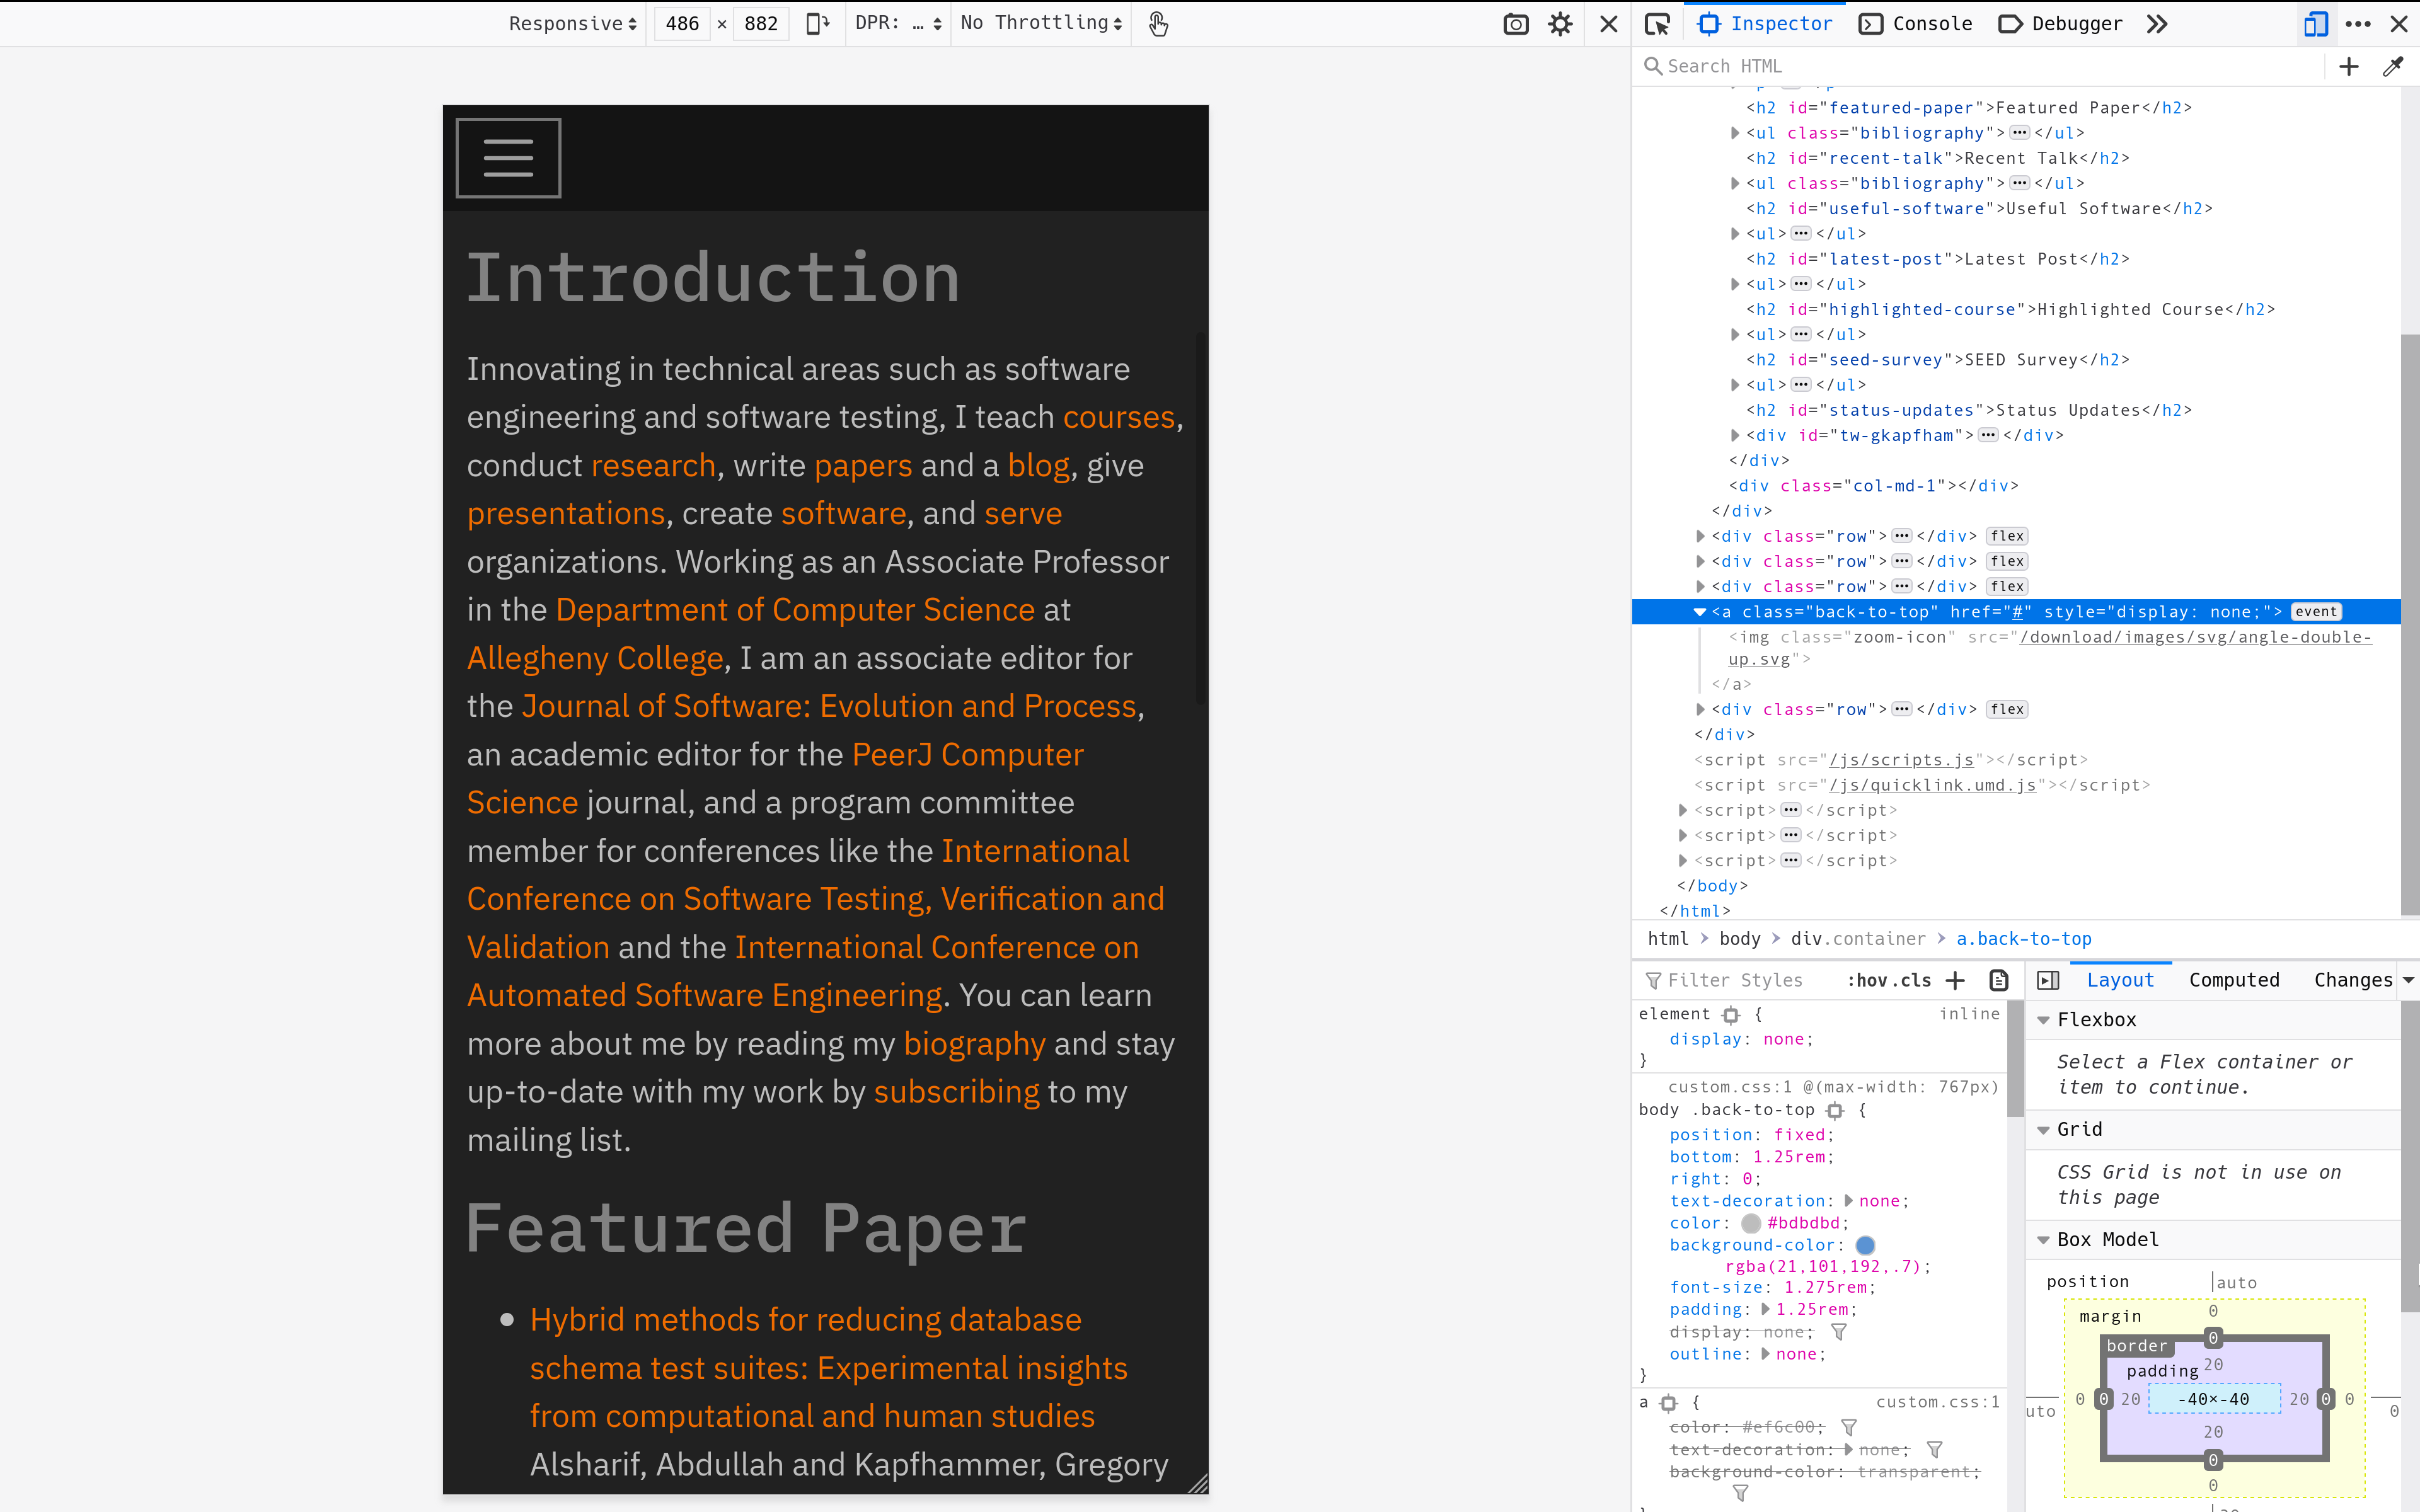
\includegraphics[scale=.085]{images/responsive-mode-firefox.png}
    \caption{The figure's caption}
  \end{figure}
  %
\end{frame}

\end{document}
